\chapter{Methane combustion simulation with Julia} \label{ch:methane}

Julia is still relatively new with a 9-year history as of 2021. Despite the recent development of Julia's ecosystem, its application in combustion modelling remains to be explored. In order to examine the its capability, we start from simple combustion simulation of methane before modelling real physical networks. It is also important to test the correctness of Julia's packages by comparing results from other programming languages.

\section{One-step mechanism}

The one-step reaction mechanism of methane combustion is described in section~\ref{sec:methane_mechanism}. The package ModelingToolkit.jl is used in combination with DifferentialEquations.jl to define the ordinary differential equations of the mathematical model. \textcite{methane_python} adopted the forward Euler scheme with Python to simulate the reaction. The parameters and initial conditions are kept the same which are summarized in table~\ref{tab:one-step}. The Julia implementation can be found in appendix~\ref{app:one-step} on page~\pageref{app:one-step}. The results shown in figure~\ref{fig:one-step} are the same which indeed demonstrate the basic functions of DifferentialEquations.jl and ModelingToolkit.jl.

\begin{table}[ht!]
\centering
\begin{tabular}{l l l} 
 \hline
 Parameters and inputs & \multicolumn{2}{l}{Values} \\
 \hline
 Activation energy $E_a$ & \multicolumn{2}{l}{$2 \times 10^4$} \\
 Temperature exponent $\beta$ & \multicolumn{2}{l}{0.0} \\
 Pre-exponential factor $A$ & \multicolumn{2}{l}{$1.1 \times 10^{10}$} \\
 Reaction exponents & $n_{\ce{CH4}}$ & 1.0 \\
 & $n_{\ce{O2}}$ & 0.5 \\
 Start time $t_0$ & \multicolumn{2}{l}{0.0} \\
 End time $t_n$ & \multicolumn{2}{l}{$2 \times 10^{-8}$} \\
 Constant temperature $T$ & \multicolumn{2}{l}{1000} \\
 Initial values & $[\ce{CH4}]$ & 1.0 \\
 & $[\ce{O2}]$ & 2.0 \\
 & $[\ce{CO2}]$ & 0.0 \\
 & $[\ce{H2O}]$ & 0.0 \\
 \hline
\end{tabular}
\caption{Parameters and inputs for the one-step reaction mechanism of methane combustion}
\label{tab:one-step}
\end{table}

\begin{figure}[ht!]
    \centering
    \begin{subfigure}[b]{0.48\textwidth}
        \includesvg[width=\textwidth]{images/one_step_mechanism_methane}
        \caption{Julia}
        \label{fig:one-step-julia}
    \end{subfigure}
    ~ %add desired spacing between images, e. g. ~, \quad, \qquad, \hfill etc. 
      %(or a blank line to force the subfigure onto a new line)
    \begin{subfigure}[b]{0.48\textwidth}
        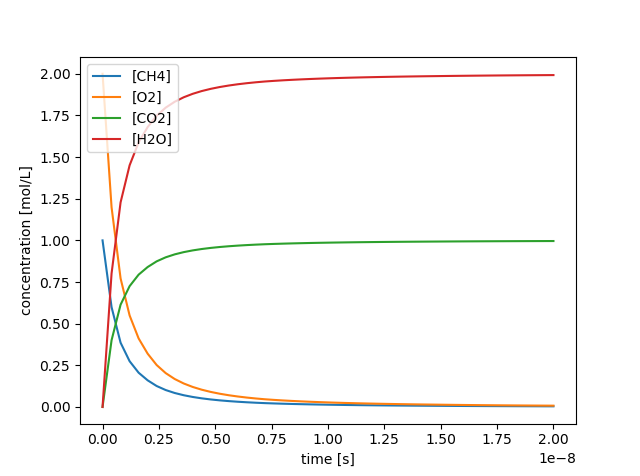
\includegraphics[width=\textwidth]{images/one-step-python.png}
        \caption{Python \parencite[p.~26]{methane_python}}
        \label{fig:one-step-python}
    \end{subfigure}
    \caption{One-step mechanism of methane combustion}\label{fig:one-step}
\end{figure}

\section{Two-step mechanism}

The combustion of methane is actually a sequence of elementary reactions rather than the straightforward one-step mechanism. The 2S\_CH4\_BFER scheme by \textcite{FRANZELLI2012621} considered in this section is explained in subsection~\ref{subsec:CO}. We would like to find an approximation solution to the following model for $0 < t < 10^{-7}$.
\begin{subequations}
\begin{align}
    \frac{\mathrm d [\ce{CH4}]}{\mathrm d t} &= - k_1 , \\
    \frac{\mathrm d [\ce{O2}]}{\mathrm d t} &= - 1.5k_1 - 0.5k_2 , \\
    \frac{\mathrm d [\ce{CO}]}{\mathrm d t} &= k_1 - k_2 , \\
    \frac{\mathrm d [\ce{CO2}]}{\mathrm d t} &= k_2 , \\
    \frac{\mathrm d [\ce{H2O}]}{\mathrm d t} &= 2k_1 .
\end{align}
\end{subequations}

The same parameters in table~\ref{tab:CO_k} on page~\pageref{tab:CO_k} are applied. We begin from the simulation with the initial conditions in table~\ref{tab:two-step-inputs} to compare the solutions with the existing Python implementation. 

\begin{table}[ht!]
\centering
\begin{tabular}{l c} 
 \hline
 Species & Initial values \\
 \hline
 \ce{CH4} & 1.0 \\
 \ce{O2} & 2.0 \\
 \ce{CO} & 0.0 \\
 \ce{CO2} & 0.0 \\
 \ce{H2O} & 0.0 \\
 \hline
\end{tabular}
\caption{Inputs for the two-step reaction mechanism of methane combustion}
\label{tab:two-step-inputs}
\end{table}

\begin{figure}[ht!]
    \centering
    \begin{subfigure}[b]{0.38\textwidth}
        \includesvg[width=\textwidth]{images/two_step_mechanism_methane}
        \caption{Julia}
        \label{fig:two-step-julia}
    \end{subfigure}
    ~ %add desired spacing between images, e. g. ~, \quad, \qquad, \hfill etc. 
      %(or a blank line to force the subfigure onto a new line)
    \begin{subfigure}[b]{0.58\textwidth}
        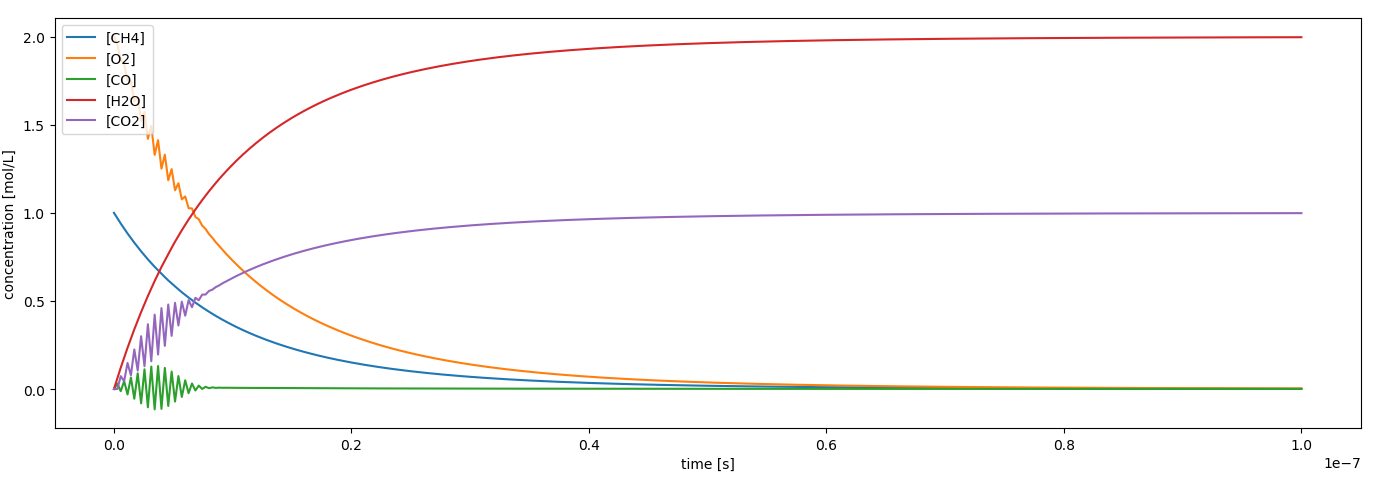
\includegraphics[width=\textwidth]{images/two-step-python.png}
        \caption{Python \parencite[p.~28]{methane_python}}
        \label{fig:two-step-python}
    \end{subfigure}
    \caption{Two-step mechanism of methane combustion}\label{fig:two-step}
\end{figure}

The results in figure~\ref{fig:two-step} look the same for both implementations except the small fluctuation in Python's figure~\ref{fig:two-step-python} due to the numerical methods it adopted. Note that while we are investigating pollutant formation, it is not particularly obvious from the figure that the carbon monoxide (\ce{CO}) is produced. Figure~\ref{fig:two-step-CO} is a separate graph for \ce{CO}. The concentration of \ce{CO} jumps sharply away from 0 immediately after the reaction starts.

\begin{figure}[ht!]
    \centering
    \includesvg[width=0.8\textwidth]{images/two_step_mechanism_methane_CO}
    \caption{Carbon monoxide in two-step mechanism of methane combustion}
    \label{fig:two-step-CO}
\end{figure}